% https://es.overleaf.com/latex/templates/project-report/jpzczmpsdzwm

%%% Preamble
\documentclass[paper=leter, fontsize=11pt]{scrartcl}
\usepackage[utf8]{inputenc}
\usepackage[spanish,mexico]{babel}
\usepackage[T1]{fontenc}    % use 8-bit T1 fonts
\usepackage{lmodern}
\usepackage{hyperref}       % hyperlinks
\usepackage{lipsum}
\usepackage[square,numbers]{natbib}

\usepackage[protrusion=true,expansion=true]{microtype}	
\usepackage{amsmath,amsfonts,amsthm} % Math packages
\usepackage[pdftex]{graphicx}
\usepackage{url}
 
\usepackage{booktabs}
\usepackage[table,xcdraw]{xcolor}

\usepackage{tikz}
\usetikzlibrary{positioning,matrix, arrows.meta}

\usepackage{caption} 
\usepackage{subcaption}


\usepackage{listings}
\lstdefinestyle{mystyle}{ 
    basicstyle=\ttfamily\footnotesize,
    breakatwhitespace=false,         
    breaklines=true,                 
    captionpos=b,                    
    keepspaces=true,                 
    numbers=left,                    
    numbersep=5pt,                  
    showspaces=false,                
    showstringspaces=false,
    showtabs=false,                  
    tabsize=4
}

\lstset{style=mystyle}
\renewcommand{\lstlistingname}{Código}


\selectlanguage{spanish}
\usepackage[spanish,onelanguage,ruled]{algorithm2e}


%%% Custom sectioning
\usepackage{sectsty}
\allsectionsfont{\centering \normalfont\scshape}


%%% Custom headers/footers (fancyhdr package)
\usepackage{fancyhdr}
\pagestyle{fancyplain}
\fancyhead{}											% No page header
\fancyfoot[L]{}											% Empty 
\fancyfoot[C]{}											% Empty
\fancyfoot[R]{\thepage}									% Pagenumbering
\renewcommand{\headrulewidth}{0pt}			% Remove header underlines
\renewcommand{\footrulewidth}{0pt}				% Remove footer underlines
\setlength{\headheight}{13.6pt}


%%% Equation and float numbering
\numberwithin{equation}{section}		% Equationnumbering: section.eq#
\numberwithin{figure}{section}			% Figurenumbering: section.fig#
\numberwithin{table}{section}				% Tablenumbering: section.tab#


%%% Maketitle metadata
\newcommand{\horrule}[1]{\rule{\linewidth}{#1}} 	% Horizontal rule

%%% https://tex.stackexchange.com/a/118217
\usepackage{mathtools}
\DeclarePairedDelimiter\ceil{\lceil}{\rceil}
\DeclarePairedDelimiter\floor{\lfloor}{\rfloor}

\usepackage{amsmath}

\usepackage{tikz}

\title{
		%\vspace{-1in} 	
		\usefont{OT1}{bch}{b}{n}
		\normalfont \normalsize \textsc{Posgrado de Ingeniería de Sistemas} \\ [25pt]
		\horrule{0.5pt} \\[0.4cm]
		\huge Pruebas estadísticas \\
		\horrule{2pt} \\[0.5cm]
}
\author{
		\normalfont 								\normalsize
        Alberto Benavides\\[-3pt]		\normalsize
        \today
}
\date{}


%%% Begin document
\begin{document}
\maketitle

\section{Preguntas}

\subsection{¿Relación entre contraste de hipótesis y pruebas estadísticas?}
Un contraste de hipótesis es un procedimiento en el que se prueba si una población se comporta como se espera a partir de una hipótesis. Existen dos tipos de hipótesis, la \emph{hipótesis nula} $H_0$ que se quiere comprobar, y la \emph{hipótesis alternativa} $H_1$ que se contrasta con $H_0$. Las pruebas estadísticas ayudan a probar estas hipótesis mediante procedimientos que permiten aceptarlas o rechazarlas a partir de intervalos de confianza, comparaciones entre medias, regresiones, etc.

\subsection{¿Qué indicaría rechazar la hipótesis nula?}
Dependiendo del intervalo de confianza, indicaría que no es verdadera o que no se tienen suficientes datos para aceptarla como verdadera.

\subsection{¿Cómo se interpreta la salida de una prueba estadística?}
Generalmente se interpreta con un valor $p$ que indica la probabilidad de que los resultados obtenidos por muestreo de la población estudiada sobre la o las variables de interés coincidan con los de $H_0$, de modo que obtener valores menores a un $\alpha$ dado, generalmente de $0.05$, se traduciría en que es casi imposible que las muestras de la población tengan valores similares a los de $H_0$, por lo que se rechazaría ese supuesto.

\subsection{¿Cómo seleccionar el $\alpha$?}
El valor de $\alpha$ generalmente se establece en $0.05$, sin embargo pueden usarse otros valores como $0.1$ o $0.01$ dependiendo del tipo de problema.

\subsection{¿Cuáles son los errores frecuentes de interpretación del valor $p$?}
Son dos y se les llama \emph{error tipo I} y \emph{error tipo II}. El primero consiste en rechazar la hipótesis nula cuando ésta es verdadera y el segundo en aceptar la hipótesis nula cuando es falsa.

\subsection{¿Qué es la potencia estadística y para qué sirve?}
La potencia estadística se utiliza para calcular la probabilidad de rechazar la hipótesis nula cuando la hipótesis alternativa es verdadera. Si se denomina $\beta$ la probabilidad de ocurrencia de un error de tipo II, entonces la potencia estadística es $1 - \beta$.

\subsection{Ejemplos de pruebas estadísticas paramétricas y no paramétricas.}
\begin{itemize}
    \item Paramétricas:
    \begin{itemize}
        \item Prueba t;
        \item análisis de varianza;
        \item correlación lineal.
    \end{itemize}
    \item No paramétricas
    \begin{itemize}
        \item Wilcoxon,
        \item Mann Whitney,
        \item Kruskal Wallis.
    \end{itemize}
\end{itemize}

\subsection{¿Cuáles son los supuestos para aplicar técnicas paramétricas?}
Que la población a la que se apliquen los datos debe tener una distribución normal y los errores independientes.

\section{Ejemplo}

Se aplican distintas pruebas estadísticas a dos conjuntos de datos obtenidos del SIMA \citet{sima} que contienen registros de calidad del aire para partículas de PM$10$ medidos en dos estaciones de monitoreo, la Norte y la Sur, ubicadas en Nuevo León, México en los municipios de Escobedo y Santiago, respectivamente. Una visualización de los datos en diagramas de cajas y bigotes junto a escalas de calidad del aire compartidas por el SIMA aparece en la figura \ref{boxplots} (p. \pageref{boxplots}).

\begin{figure}
    \centering
    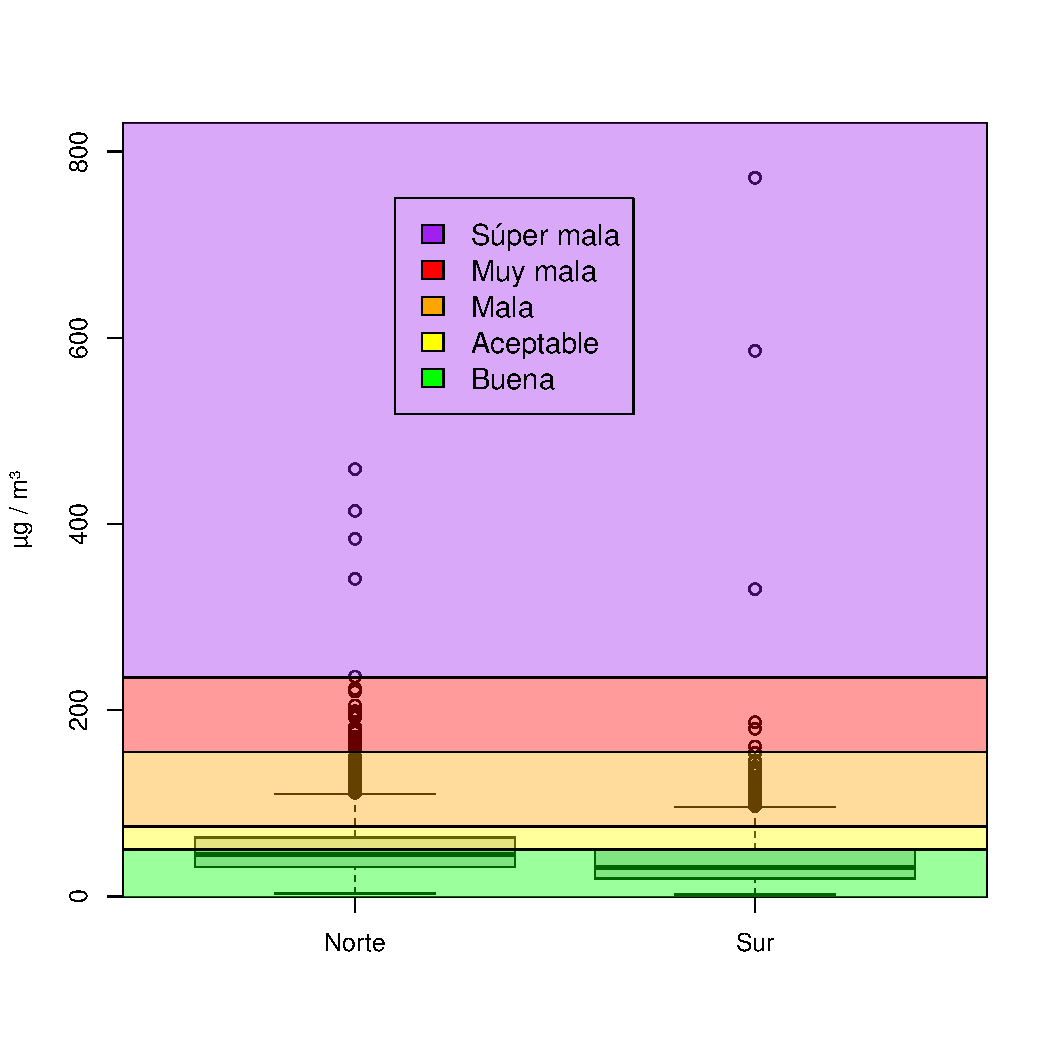
\includegraphics[width=1\textwidth]{boxplots.pdf}
    \caption{Diagramas de cajas y bigotes de las concentraciones de contaminantes con tamaño PM$10$ para las estaciones Norte y Sur durante el año 2018, medidas en $\mu\text{g}/\text{m}^3$.}
    \label{boxplots}
\end{figure}

A estos conjuntos de datos se les aplica una prueba de Shapiro para determinar si tienen distribución normal, mas es sólo con fines demostrativos, pues los histogramas ya evidencian una distribución geométrica para ambos conjuntos de datos, como se muestra en la figura \ref{hist} (p. \pageref{hist}). Los valores $p$ para ambos conjuntos de datos dan $2.2 \times 10^{-6}$ por lo que se puede rechazar la hipótesis nula de que sigan distribuciones normales.

\begin{figure}
    \begin{subfigure}{.5\textwidth}
        \centering
        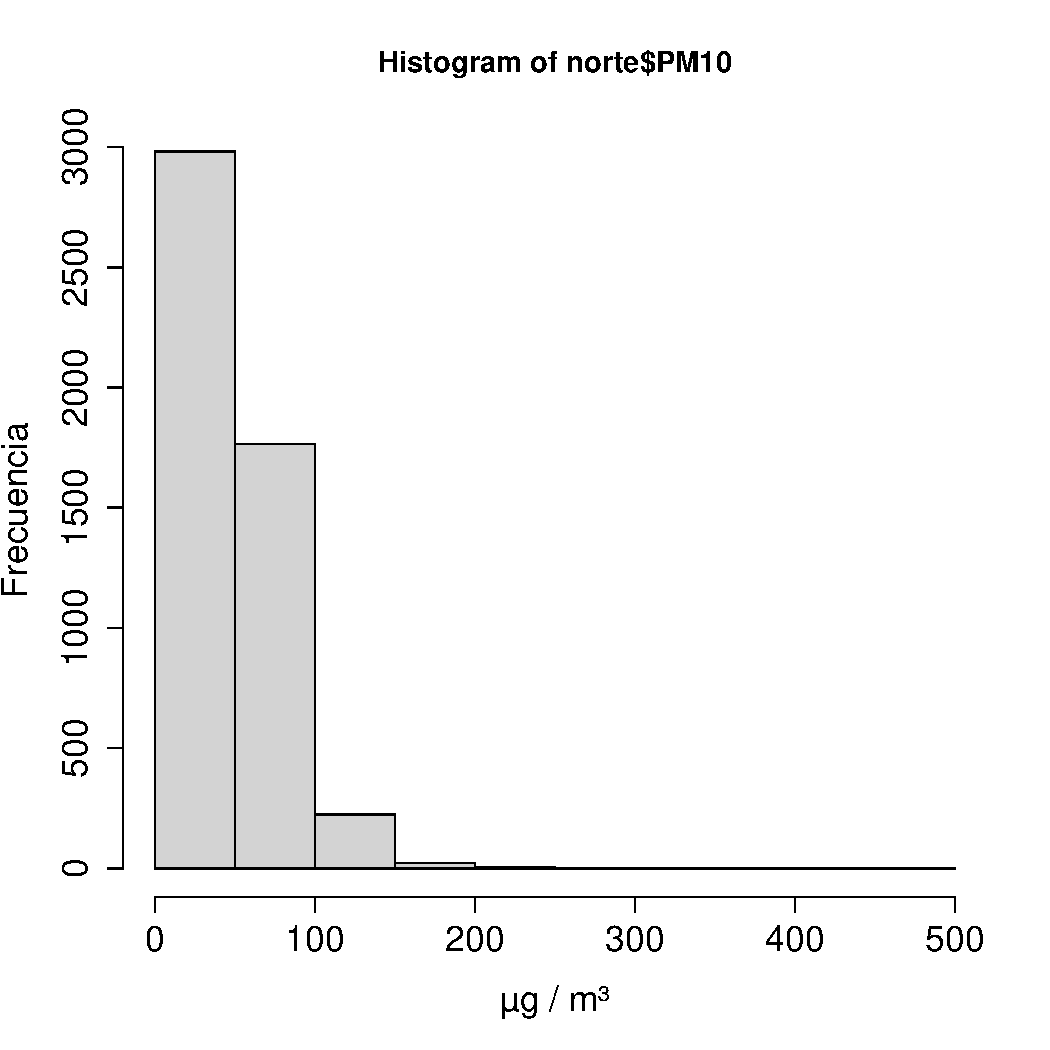
\includegraphics[scale=0.4]{norte_hist.pdf}
        \caption{Sur}
        \label{norte_hist}
    \end{subfigure}
    \begin{subfigure}{0.5\textwidth}
        \centering
        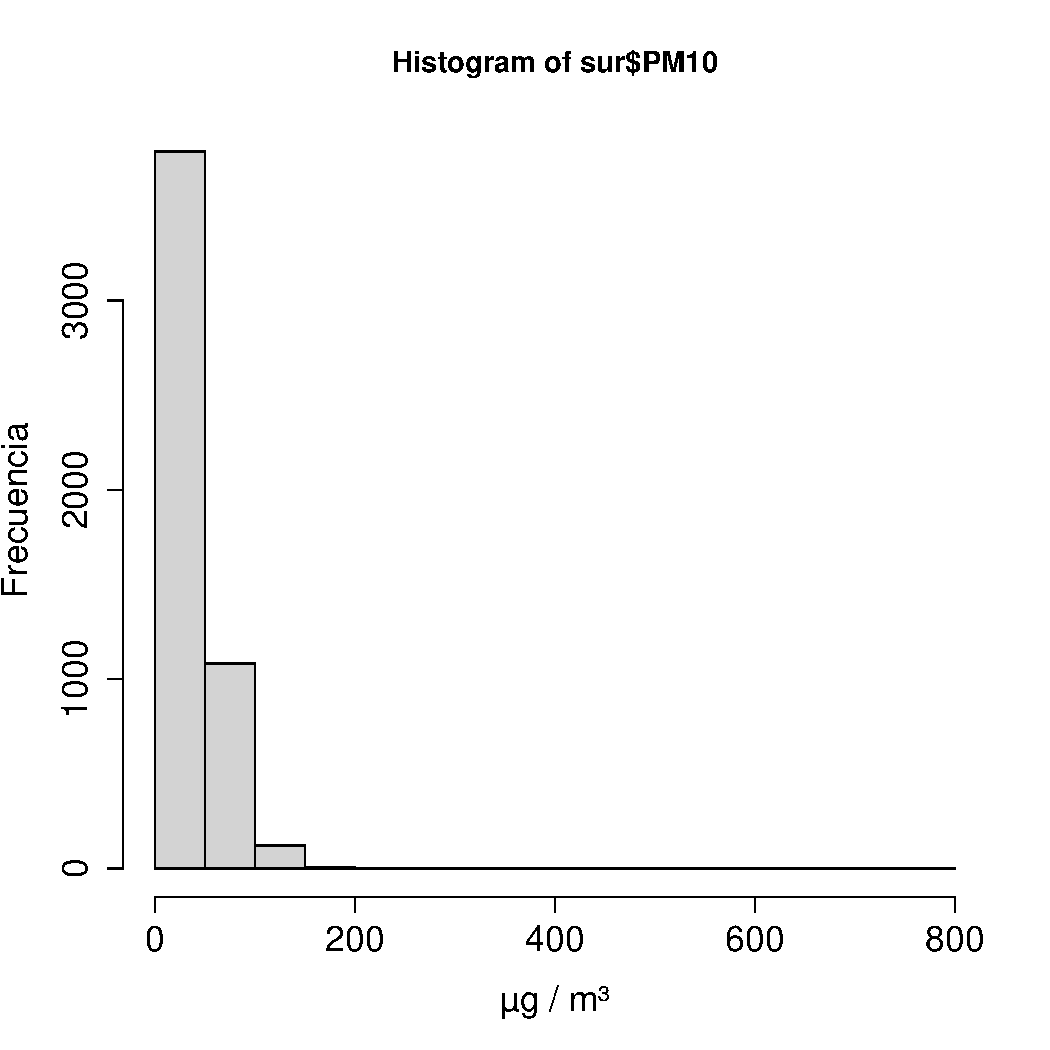
\includegraphics[scale=0.4]{sur_hist.pdf}
        \caption{Sur}
        \label{sur_hist}
    \end{subfigure}
    \caption{Histogramas para las concentraciones de contaminantes de tamaño PM$10$ para las estaciones Norte y Sur.}
    \label{hist}
\end{figure}

Ahora se utiliza una prueba para determinar si de alguno de los conjuntos de datos se puede extraer una media dada. Esto se hace mediante una prueba $t$ cuando los datos están normalmente distribuidos, pero como estos conjuntos no lo están, se utiliza la prueba de Wilcoxon. Como valor de media se elige $50$ por ser el valor máximo del rango de valores de buena calidad del aire. La prueba tiene valores $p < 0.01$ para ambos conjuntos, por lo que se puede rechazar la hipótesis nula en ambos casos, además de que estima medias para ambos conjuntos de $47\mu\text{g}/\text{m}^3$ y $34\mu\text{g}/\text{m}^3$, por lo que se podría decir que en 2018 la calidad del aire en cuanto a este tipo de contaminante fue bastante buena. Sin embargo, cuando se comparan las medias para ambos conjuntos de datos mediante Wilcoxon, con el valor $p = 2.2 \times ^{-16}$, se puede concluir que las medias son distintas, lo cual también se había constatado visiblemente en los diagramas de cajas y bigotes de la figura \ref{boxplots} (p. \pageref{boxplots}).

Ahora bien, mediante una prueba $F$ puede determinarse si ambos conjuntos tienen la misma varianza, sin embargo se puede concluir que no es así dado que el valor $p = 0.07$, por lo que se rechaza la hipótesis nula de esta prueba que supone ambas distribuciones tienen la misma varianza. Por último, resulta interesante determinar si las estaciones tienen alguna relación entre sí. Para ello se puede realizar una prueba de correlación entre ambos conjuntos que tiene como hipótesis nula que la correlación entre los conjuntos es igual a $0$. El valor $p$ obtenido para esta prueba fue $1.99 \times 10 ^{-5}$, de modo que se puede afirmar que existe alguna correlación entre los conjuntos de datos.

\bibliographystyle{plainnat}
\bibliography{Biblio}

\end{document}